	\chapter{Work Completed}

        \section{Collection of Dataset}

        In this section, we went through multiple sources in the internet and discovered different datasets in different forms. We gathered datasets from various online sources, ensuring diversity and relevance to our task. The dataset collection process involved the following steps:

        \subsection{Selection of Suitable Online Sources}
        We searched through online platforms and specialized repositories to identify suitable video and image datasets for lip reading research. Some of the datasets we came across include:

        \begin{itemize}
            \item GRID (Glasgow University Multimedia Database)
            \item LRW (Lip Reading Words) Dataset
            \item LRS2 (Lip Reading Sentences 2) Dataset
            \item MIRACL-VC1 (Multimodal Interaction in Rich Communication Channels)
        \end{itemize}

        \subsection{Data Access}
        Once the relevant datasets were identified, we accessed them through the official websites or repositories provided by the dataset creators. We ensured compliance with any usage terms and conditions specified by the dataset providers.
        
        \begin{table}[h]
            \centering
            \label{table:dataset_characteristics}
            \begin{tabular}{|l|c|c|}
                \hline
                \textbf{Dataset} & \textbf{Language} & \textbf{Number of Samples} \\
                \hline
                    GRID & English & 1000+ \\
                    MIRACL-VC1 & Multi-lingual & 500+ \\
                    LRW & English & 5000+ \\
                    LRS2 & English & 100,000+ \\
                    
                \hline
            \end{tabular}
        \caption{Characteristics of Datasets}
        \end{table}
        \section{Dataset}
        We ended up choosing to go with the GRID dataset. The dataset contains both audio and video features and 
        In this project we are only using the visual feature but in case in the future we were to extend this project to use the audio feature as well then this dataset is the better choice.
        
       \section{Landmark Identification}
       \begin{figure}[h]
	\centering
	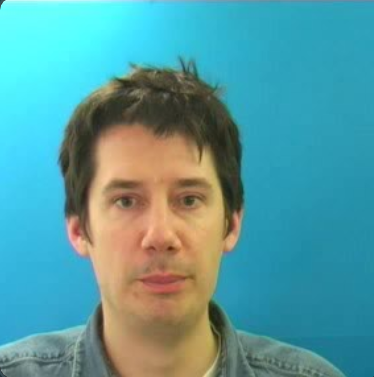
\includegraphics[width=0.4\linewidth]{img/face.png}
	\caption{Original Image}
	
	\end{figure}
 The size of the image is 360*228 and the video is of 25Fps and is 3 seconds long. In the dataset there are total of 34 talkers(18 male, 16 female) but to train our model we only used the data of one speaker.So for landmark identification we used frame slicing to separate the lip from each frame of the video. It is only possible because we used single speaker and the framing of the video is same for each data in the dataset.


 
       \begin{figure}[h]
	\centering
	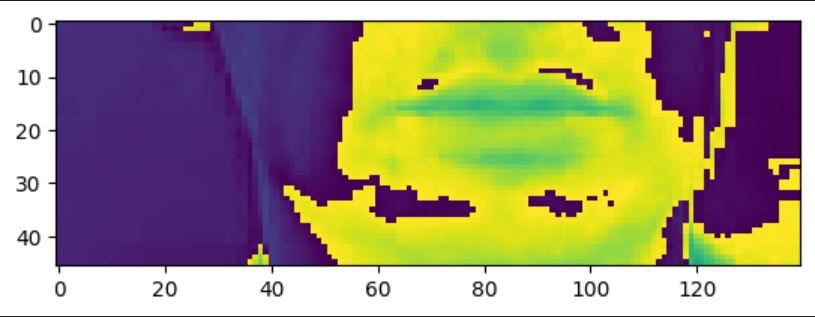
\includegraphics[width=0.6\linewidth]{img/cropped.png}
	\caption{Cropped image}
	
	\end{figure}
    \pagebreak
    
    \section{Model Architecture}
    The model consists of three blocks of 3D convolutional, ReLU activation, and 3D max pooling layers, followed by a TimeDistributed layer that flattens the output of each timestep. Then, the model has two blocks of bidirectional LSTM, dropout, and dense layers, with a softmax activation layer at the end. The model takes an input of shape (75,46,140,1) and produces an output of shape (75,27), where each element is a probability distribution over the vocabulary of characters.


\subsection{Early Performance Evaluation}
 The training was done over 50 epochs using a GCP VM having Nvidia V100 GPU having 16GB memory. Each epoch took about 8 minutes on average to train and the Loss Curve and Letter-level accuracy curve was plotted after the training of the model was completed.
    \begin{figure}[h]
	\centering
	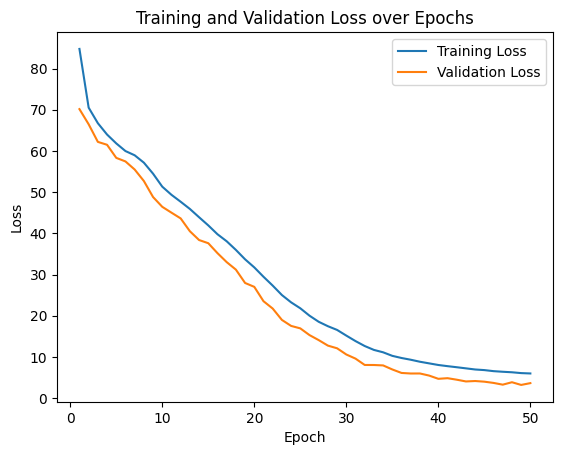
\includegraphics[width=0.6\linewidth]{img/loss.png}
	\caption{Loss Curve}
	
	\end{figure}

We observed a steady decline in the loss metric of both training and validation as the training progressed through epochs. Having said so, We believe that the model can make further improvements in performance with optimized code and improved hardware.
\pagebreak
\begin{figure}[h]
	\centering
	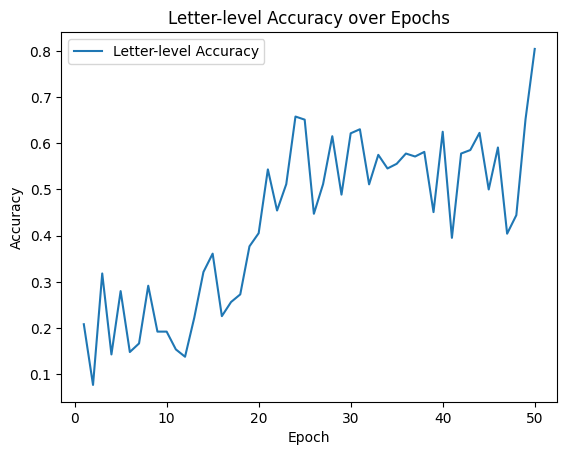
\includegraphics[width=0.6\linewidth]{img/accuracy.png}
	\caption{Letter-Level Accuracy}
	
	\end{figure}


The graph shows the letter-level accuracy of a neural network model over 50 epochs. The accuracy increases from 0 to 0.8, with a spike after epoch 40. The graph indicates that the model learns better over time and achieves a high accuracy at the end.



 
               
       

                        
        
